%*****************************************************************************************
\part{Analysis of Current System}
\chapter{Introduction and Background}
\ifpdf
    \graphicspath{{Chapter2/Figs/Raster/}{Chapter2/Figs/PDF/}{Chapter2/Figs/}}
\else
    \graphicspath{{Chapter2/Figs/Vector/}{Chapter2/Figs/}}
\fi

%%%%%%%%%%%%%%%%%%%%%%%%%%%%%%%%%%%%%%%%%%%%%%%%%%%%%%%%%%%%%%%%%%%%%%%%%%%%%%%
\section{Introduction}

This part of the project can be outlined as follows:

\begin{itemize}
    \item Collect data sets on which a machine learning classifier is to be trained
    \item Construct a program capable of processing and storing such data sets
        such that required subsets of the data can be quickly and easily
        returned for further analysis
    \item Select a suitable machine learning framework to handle the training
        and validation of a classifier
    \item Ensure a robust validation methodology exists for assuring quality of
        our own results
    \item Set up an environment capable of allowing results from such a
        classifier to be stored and compared
    \item Training a suitable classifier on the collected data sets
    \item Perform experiments by selecting subsets of the variables and
        observations and measure whether classification accuracy is improved
\end{itemize}


%%%%%%%%%%%%%%%%%%%%%%%%%%%%%%%%%%%%%%%%%%%%%%%%%%%%%%%%%%%%%%%%%%%%%%%%%%%%%%%
\section{Concepts and Terminology}
\subsection{Whole Genome Sequencing}
...the process of recovering the sequence of bases called nucleotides...

\subsection{Samples, Lanes and Lanelets}
\label{chap:samplelanelanelets}

%TODO Draw a vector of the lanelets diagram
%TODO Illumina DNA Synthesis Image
A \textbf{sample} is a distinct DNA specimen extracted from a particular person.
For the purpose of sequencing, samples are then pipetted in to a
\textit{flowcell} such as the one in Figure~\ref{fig:flowcell} --- a glass slide
containing a series of very thin tubules known as \textbf{lanes}.  It is
throughout these lanes that the chemical reactions involved in sequencing will
take place.

\begin{figure}[htbp!]
    \centering
    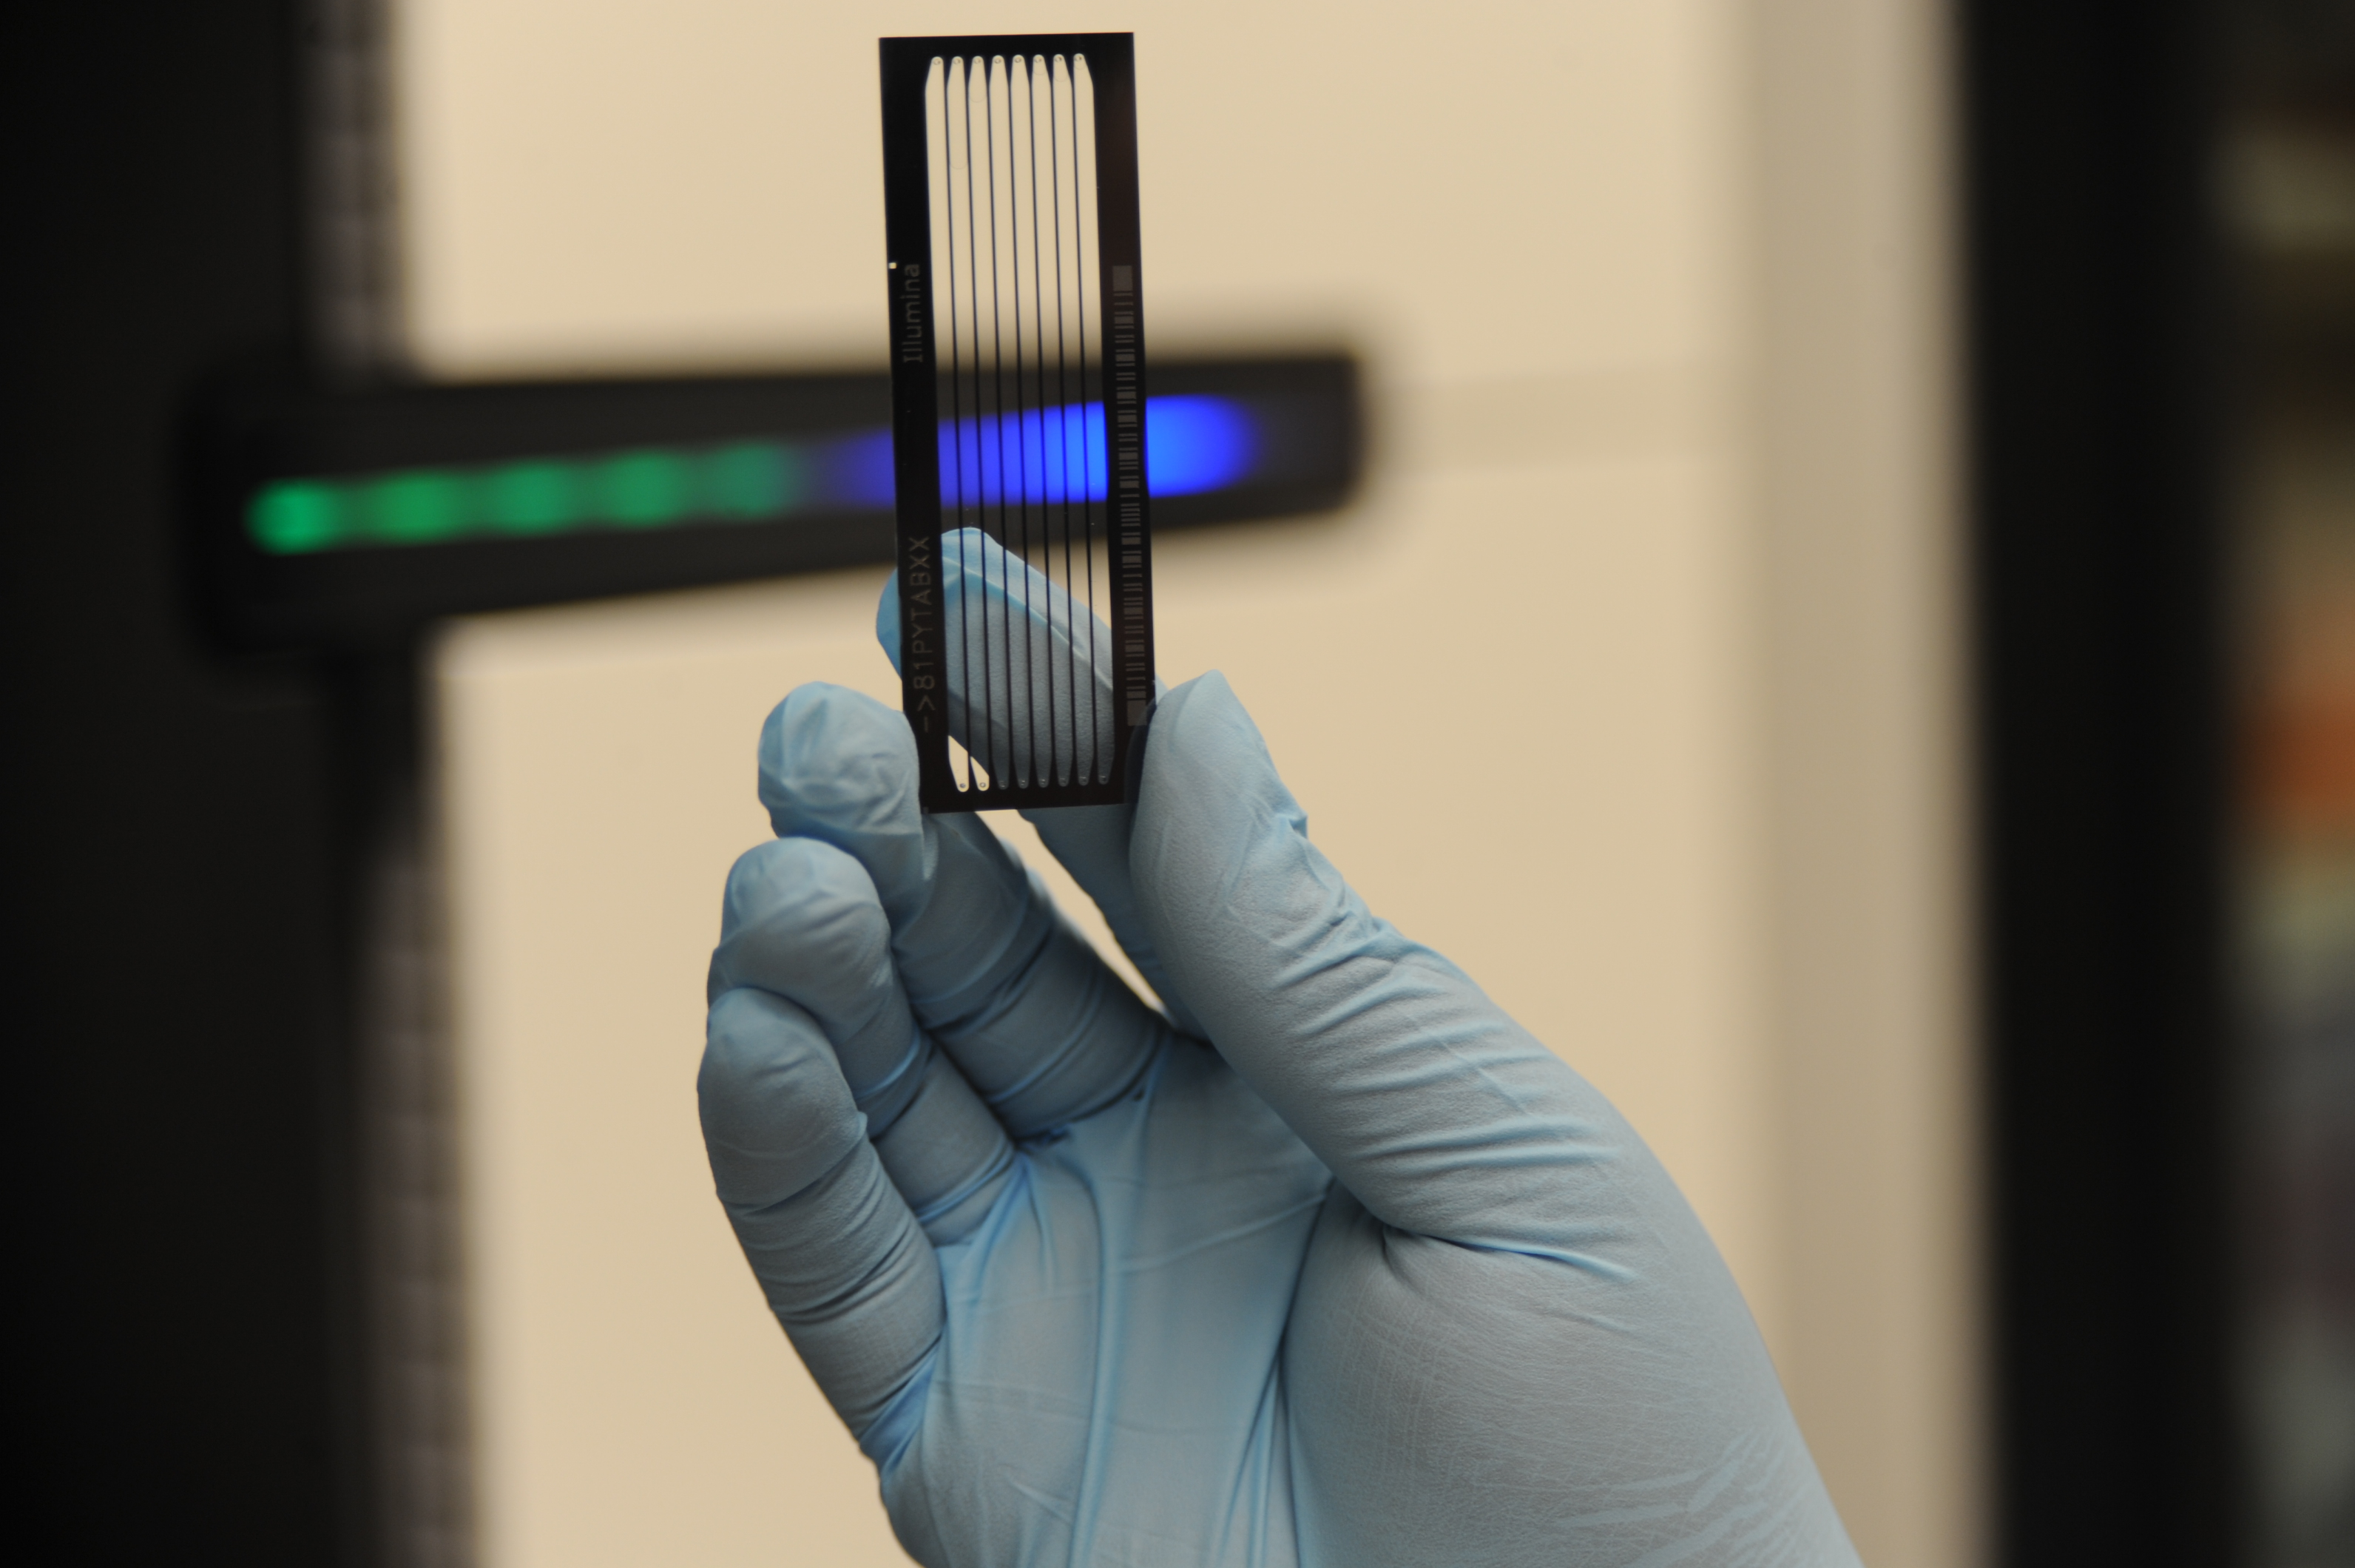
\includegraphics[width=0.4\textwidth]{NHGRI-80102}
    \caption[flowcell]{An Illumina HiSeq Flowcell\citep{img:flowcell}}
    \label{fig:flowcell}
\end{figure}

Once inserted, samples are amplified in situ inside the flowcell itself whereby
samples multiply in magnitude to form millions of dense clusters. Note that a
lane can contain more than one sample and a sample can appear in more than one
lane; this is "sample multiplexing" and helps to ensure that the failure of a
particular lane does not hinder analysis of a sample.

A \textbf{lanelet} is the aggregate read of all clusters of a particular sample
in a single lane. Figure~\ref{fig:lanelets} attempts to highlight examples of a
this (circled in blue - not all lanelets are highlighted). For example lane 5
shows the four clusters (in reality there would actually be millions) of Sample
A combine to represent a lanelet. A lane will have as many lanelets as it does
samples.

\begin{figure}[htbp!]
    \centering
    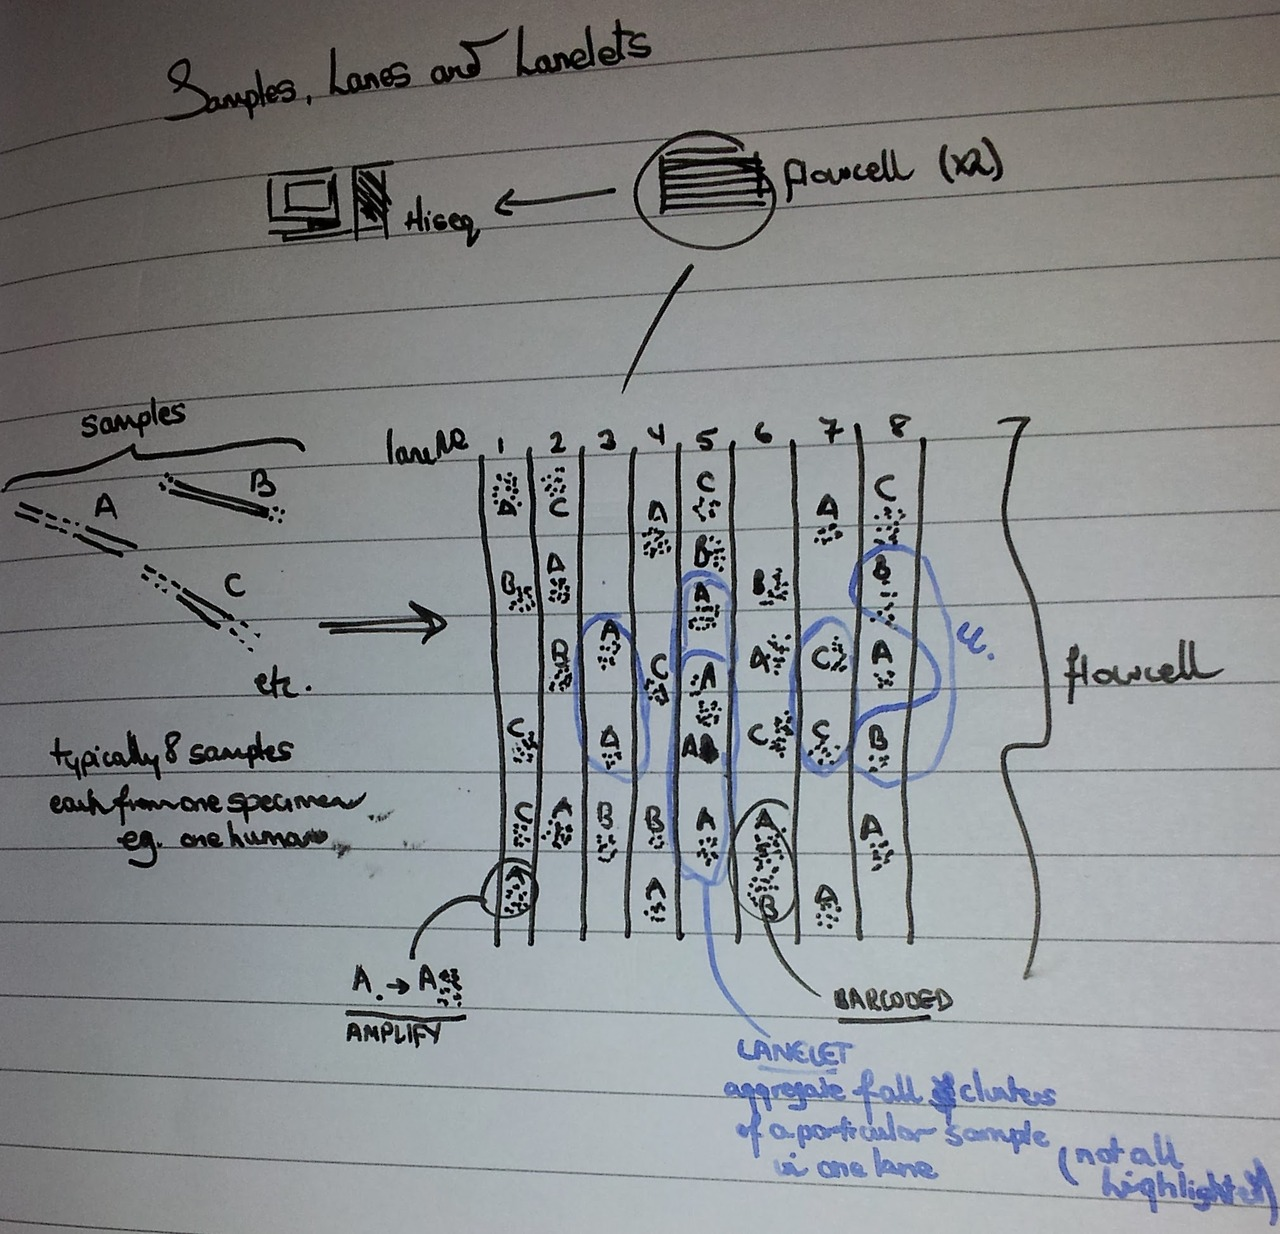
\includegraphics[width=0.5\textwidth]{lanelets}
    \caption[lanelets]{Example of flowcell with some lanelets highlighted}
    \label{fig:lanelets}
\end{figure}


%%%%%%%%%%%%%%%%%%%%%%%%%%%%%%%%%%%%%%%%%%%%%%%%%%%%%%%%%%%%%%%%%%%%%%%%%%%%%%%
\chapter{Materials and Methods}
\section{Input Data and Format}
\subsection{"BAMcheckR'd" Data}
\label{chap:bamcheckr-data}

%NOTE Assuming lanelets have been described by this point...
%TODO samtools stats actually generates this data rather than "the seq process"
As part of the project I've been granted access to significant data sets at the
Sanger Institute, unlocking quality control data for two of the largest studies
currently undergoing analysis. A wide array of quality metrics are available for
each and every lanelet that forms part of either of the two studies; totalling
13,455 files.

%9154 (68\%), 1542 (11\%), 2759 (21\%)...

%TODO Explain a BAM file
The files are created by \textbf{samtools stats} --- part of a collection of
widely used open-source utilities for post processing and manipulation of large
alignments such as those produced by next-generation sequencers that are
released under the umbrella name of "SAMtools"\citep{samtools} (Sequence Alignment and Map
Tools). \textbf{samtools stats} collects statistics from sequence data files %BAM
and produces key-value summary numbers as well as more complex tab delimited
dataframes tabulating several metrics over time.

%TODO Was samtools stats known as bamcheck, or did it replace it?
The output of \textbf{samtools stats} is then parsed by an in-house tool called
\textbf{bamcheckr}, named so as \textbf{samtools stats} was once known as
\textbf{bamcheck} and the tool is written in R. \textbf{bamcheckr} supplements
the summary numbers section of the \textbf{samtools stats} output with
additional metrics that are later used by \textbf{auto\_qc} for classification.
This process does not change the file other than adding a few additional
key-value pairs in the summary numbers section. A truncated example of a
"bamcheckr'd" file can be found in Appendix~\ref{app:bamcheckr}.

\subsection{auto\_qc Decision Data}
To use these "bamcheckr'd" files for training and testing a machine learning
classifier, it is necessary to map each file to a classification result from
\textbf{auto\_qc}. The one-to-one mapping between each input file and its label
are provided by the Sanger Institute in a separate file hereafter referred to as
the \textit{AQC Decision Matrix} or \textit{AQC (Decision) File}.

A truncated example of such a file can be found in Appendix~\ref{app:aqc_matrix}.
Only the first few columns are included --- indeed we are only interested in the
\textit{lanelet} and \textit{aqc} which provide an identifier that maps the row
to a given input file and its classification by \textbf{auto\_qc} respectively.
Latter columns pertain to a breakdown of decisions made by \textbf{auto\_qc}
which are not included in the example for confidentiality (and brevity).


%%%%%%%%%%%%%%%%%%%%%%%%%%%%%%%%%%%%%%%%%%%%%%%%%%%%%%%%%%%%%%%%%%%%%%%%%%%%%%%
\section{Development Environment}
\subsection{Language}
%TODO Better opening
%TODO Do I need to ramble about why vim is great and so on?
For the language of the program designed to handle this vast array of input
data, Python was selected, more out of personal taste rather than a
detailed analysis of required performance and features. From previous experience
I was happy with the performance of Python when processing large datasets in
terms of both I/O file handling operations and storing the data in memory for
later use. Python's generous choice of both built-in and third-party libraries
have proven useful on many occasions. Due to its concise and flexible nature it
is possible to rapidly develop applications and its readability eases ongoing
maintenance; useful given the short time-span allocated for this project and the
possibility of others wishing to contribute to the project codebase after
completion.

Whilst the choice was made primarily on preference, this is not to say other
options were not considered: a highly popular Java-based collection of data
mining tools, \textbf{WEKA}\citep{weka} would certainly have provided a
framework for building decision tree classifiers but at the same time did not
appear to offer any significant features that were unavailable elsewhere, whilst
Java itself has the added constraint of requiring a virtual machine to be
installed which could be undesirable from a performance or even security
standpoint when the application is deployed to servers at the Sanger Institute.

%...although performance has improved considerably from previous Java versions\citep{Bouckaert}

Difficulty was also encountered finding example implementations for \textbf{WEKA}
with most documentation and tutorials providing information for performing
analysis via the graphical "Explorer" interface instead, which would not be
appropriate for quickly setting up and repeating experiments automatically.

Given the quality data we'll be using to train a machine learning classifier is
output from the previously mentioned R script; \textbf{bamcheckr}, it was worth
briefly investigating the options available for R itself as the potential of
integrating the learning and predicting functions right in to the same process
that outputs the data seemed convenient.

Whilst the \textbf{tree}\citep{man:rtree} and \textbf{rpart}\citep{man:rpart}
packages are available for constructing decision trees in R (and actually
\textbf{RWeka} provides an R interface to \textbf{WEKA}) neither appeared to be
as robust as other more well-known frameworks. Also putting it politely, the
programming paradigm of R\citep{man:R} is rather different to other languages
and can significantly increase development time (and frustration\citep{argh}) if
one is not very well versed in the patterns and grammar of the language  and it
seemed best to stick to one's comfort zone given the brief timescale for the
project.

%TODO Cite dlib, Shark
Had performance been a critical decision factor, lower level languages such as
C, C++ or even Fortran could be used. Briefly looking at two popular frameworks
available for C in particular; \textbf{dlib} did not support tree-based
classifiers although an alternative, \textbf{Shark} did.


\subsection{Framework}

Having studied the \textit{Machine and Intelligent Learning} module in final
year, the prospect of getting stuck in to the deep of a machine learning
algorithm was exciting. However the reality is that a lot of cumulative time and
effort has gone in to creation and optimisation of a framework which is unlikely
to be surpassed successfully by a short-term one-person project. Thus
utilisation of a third party machine learning library would seem a wise
investment for the project's codebase.

There are numerous machine learning frameworks available in many languages, some
of which were described above and formed part of the development environment
decisions. Whilst it is obviously not necessary to select a framework which uses
the same language as the project, it seemed counter-intuitive to select otherwise,
for the establishing of additional arbitrary output and input steps to move data
between the two environments could impede quick experiment repeatability and
introduce error.

...A mixed bag of machine learning frameworks exist in Python, two in particular
\textbf{scikit-learn}\citep{scikit-learn} and \textbf{Orange}\citep{orange}
were main contenders, partly on their recommendation from the project
supervisor.

...scikit integrates the "big names" in Python: numpy, scipy and matplotlib
...put off from Orange due to difficulties in reading in data ...it did however
later appear to ship with features that were not in scikit (pruning and
printing) ...with more time I'd certainly like to investigate using other
libraries such as \textbf{Orange} or even outside Python and take at look at WEKA
or Shark...

\subsection{Additional External Libraries}
%TODO Ref num,sci,matplot
numpy\citep{numpyscipy} and scipy\citep{scipy}... Fast and reliable implementations of
mathematical functions...  ggplot2\citep{ggplot2} for beautiful graphing...


%%%%%%%%%%%%%%%%%%%%%%%%%%%%%%%%%%%%%%%%%%%%%%%%%%%%%%%%%%%%%%%%%%%%%%%%%%%%%%%
\subsection{Testing}

As discussed in Chapter~\ref{chap:methodology}, testing forms a critical part of
the project given the need to monitor the impact of changes to classification
accuracy as well as to ensure the program is working correctly. Ideally,
execution of a test suite should be simple and easily repeatable, results that
pertain to accuracy should also be stored for future reference to monitor
ongoing performance of the classifier.

%TODO Cite Jenkins, Travis, Wercker
Such requirements could be fulfilled by a continuous integration platform; a
server dedicated to the building and testing of the code contained in a
centralised repository typically to which an entire team will have write
access\citep{fowler-ci}. Whilst in this scenario there will be much less "risk"
from integration issues due to the single person team size, the themes of
automated building and self-testing code can be taken on board.

\textbf{Jenkins} is a highly popular\cite{jenkins-stats} example of such a
platform with which I am familiar. Although an out-of-the-box Jenkins set-up is
suitable for variety of software engineering projects, it would be necessary to
invest some time to install and tweak plugins to perform actions on test results
(such as failing a build that causes accuracy to decrease). However, previous
experience found that highly specific tasks will often require a plugin to be
authored to overcome limitations in the feature set of a more generic plugin,
which given the intricacies of the Jenkins package layout could easily
turn in to a project of its own. Unfortunately, other features that would be
useful to the project including the indexing and searching of build logs are
somewhat lacking in Jenkins.

Online solutions such as \textbf{Travis} and \textbf{Wercker} could potentially
offer a quicker set up as both merely requires a small configuration file in the
root of the repository and a hook to be registered...
...however such services would
not have been able to handle artifacts such as dot files without some convoluted
solution of uploading them to dropbox or adding them to a private git repository
from the build node...  ...also would have needed to upload a very large
quantity of training data repeatedly which would be inefficient (and more than
likely against reasonable use of the platform)

Really wanted to write my own solution for this but had to settle for well
formatted log files that could be searched and processed with some command line
fu...

\subsection{Tools}
Version control is critical, \textbf{git}!


%%%%%%%%%%%%%%%%%%%%%%%%%%%%%%%%%%%%%%%%%%%%%%%%%%%%%%%%%%%%%%%%%%%%%%%%%%%%%%%
%TODO Rubbish section title
\chapter{Pre-Implementation}
\section{Classification Correlation}

%TODO Lanelet...
An important consideration for statistical analysis is the relation between
observations. The "bamcheckr'd" input data described in
Chapter~\ref{chap:bamcheckr-data} is available per lanelet, however as shown in
Chapter~\ref{chap:samplelanelanelets} a lane may contain more than one lanelet.
Herein lies the trouble; if during a sequencing run the flowcell is somehow
subjected to abnormal conditions (a temperature increase due to an air
conditioning failure) or the device is depleted of reagents then every lane (and
thus all lanelets within) will be of very poor quality.

%TODO Probably mention in the text this is a very dense heatmap...
\begin{figure}[htbp!]
    \centering
    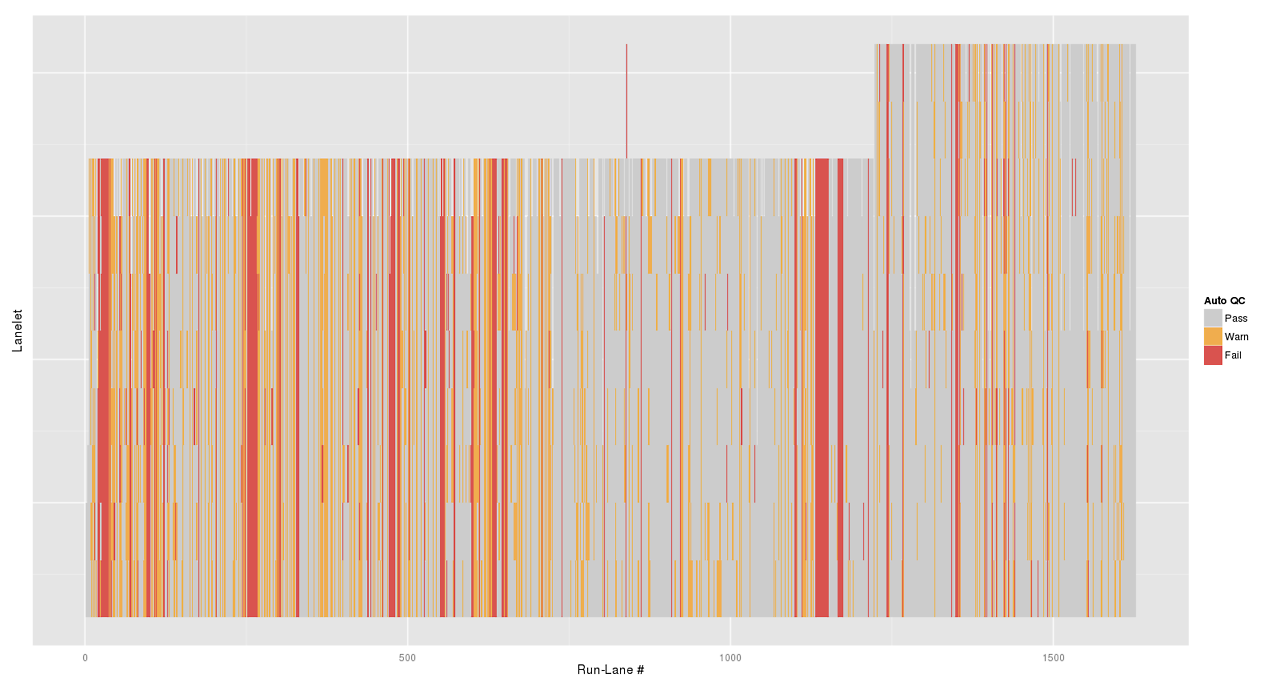
\includegraphics[width=1.0\textwidth]{classcorr}
    \caption[ClassCorr]{\textbf{Heatmap of Lanelet QC Status by Lane}: Lanes are
    Vertical bars with each lanelet cell coloured red to represent a failure,
yellow for a warning and grey for a pass.}
    \label{fig:classcorr}
\end{figure}

%TODO affected effected?
In such a case there would appear to exist a relationship between the respective
qualities of each lanelet in a lane as well as each lane in a sequencing run. To
examine this further, an R script utilising \textbf{ggplot2} was authored to
visually inspect whether correlation existed and if so to what degree that data
is affected.

Figure~\ref{fig:classcorr} displays a plot of \textbf{auto\_qc} classification
for each lanelet in a lane. The plot itself is a dense heatmap
where each lane stands as a vertical bar, broken in to horizontal cells, each
of which represents a lanelet that was sequenced in that particular lane. These
lanelets are colour coded using; red for failures, yellow for warnings and grey
for passes (to allow the other two classes to be more easily seen).

Therefore an unbroken vertical red line indicates that all lanelets that
comprise of that line failed to pass \textbf{auto\_qc}. In reality there are few
conditions under which a lanelet would fail irrespective of the auto


 I should mention that it seems there are
few conditions under which a lanelet would fail irrespective of the auto\_qc
status of the rest of the lanelets in the lane; which mostly involve the
preparation of the sample (which is easy to spot given it will cause poor
quality across all lanelets using that library sample).
for each lanelet (y) versus lane (x).

...an unbroken vertical red bar indicates that all the lanelets inside a
particular lane failed. Likewise yellow represents a warning. Grey areas are
passes and were desaturated to make the other outcomes immediately obvious. It
is clear that there are patches where lanelets have failed where entire lanes
have not, but there does appear to be some correlation.

%TODO
Having discussed this with the supervisor and contacts at the Sanger Institute
we decided to continue...

Note the plot does not make a particular distinction between lanes in the same
flow cell but they are sequentially identified so the red bars of thicker-width
arguably display some failures across entire flow cells.

